\documentclass[letterpaper,12pt]{article}

% things needed to include figures
\usepackage{subfigure, graphicx}
% float must be included for the [H] to actually work
\usepackage{float}
% formulas
\usepackage{amsmath}
% Added to adjust captions
\usepackage[singlelinecheck=false]{caption}
% added to adjust margins at the suggestion of Dr. Matt
\usepackage[top=1in, bottom=1in, left=1in, right=1in]{geometry}
\usepackage{fullpage}
\title{Optical Pumping}
\author{Max Bigras and David Frawley}

\begin{document}

\maketitle

\begin{abstract}
We performed optical pumping to trap $^{85}$Rb and  $^{87}$Rb atoms. We measured the strength of an applied magnetic field and the intensity of light passing through the Rb vapor. We determined the Lande g-factor, $g_{\mathrm{f}}$, for each of the isotopes and were able to determine the ratio $g^{\mathrm{exp}}_{87}$/$g^{\mathrm{exp}}_{85}$ = $1.5 \pm 0.1$ which agrees with the accepted value $g_{87}$/$g_{85}$ = 1.5. We also observed our applied magnetic field cancel the Earth's magnetic field.
\end{abstract}

\section{Introduction}
Optical pumping is an important experimental technique that takes precise advantage of quantum selection rules to trap and manipulate atoms. We used a technique developed in the 1950s by Alfred Kastler who later won the Nobel Prize in 1966 \cite{wiki}. By careful constructing a magnetic field from pairs of Helmholtz coils, one can adjust the Zeeman energy gap and pump atoms into a trapped state. Once trapped the atoms can be manipulated in interesting and precise ways to measure quantities like the size of the Zeeman energy gap, the atom's g-factors, or the strength of an external magnetic field.


\section{Theory}
\subsection{Zeeman splitting}
When an atomic system is placed in a magnetic field it's energy levels undergo Zeeman splitting. Our atomic system consists of the two stable isotopes $^{85}$Rb and  $^{87}$Rb. A schematic for $^{85}$Rb can be seen in Figure \ref{energy_levels}. In the Rb atoms there are three magnetic moments caused by orbiting electrons, electron spin, and nuclear spin. Taking into account these moments the equation for the energy gap between adjacent levels is

\begin{equation}
E_{\mathrm{Zeeman}}= g_{\mathrm{f}} \mu_{\mathrm{B}} B
\label{zeeman}
\end{equation}
where $g_{\mathrm{f}}$ is the Lande g-factor, $\mu_{\mathrm{B}}$ is the Bohr magneton, and $B$ is the strength of the total magnetic field felt by the atom.
\begin{figure}[H]
  \includegraphics[totalheight=0.65\textwidth]{figs/energy_levels}
  \caption{Structure of the $^{85}$Rb isotope (not to scale) image from \cite{manual}}
  \label{energy_levels}
\end{figure}

\subsection{Optical pumping}

A visual description for optical pumping can be seen in Figure \ref{pumping}. Initially all the atomic states are equally populated. At this point an atom in one of the lower states can absorb  a photon and excite, following the selection rule $\Delta m_{\mathrm{F}} = +1$. To de-excite the atom emits a photon and follows the selection rule $\Delta m_{\mathrm{F}} = -1, 0, +1$. So there is some probability that $\Delta m_{\mathrm{F}}$ will be 0 or $+1$ on the way down, causing a net ``ratcheting up'' of the atoms. Now when the Rb atom falls into the $m_{\mathrm{F}} = 3$ state it can no longer excite while following the selection rules, so it is trapped. Interestingly once all the atoms are trapped they can no longer absorb photons and become transparent, shown in  Figure \ref{pumping}g.
\begin{figure}[H]
  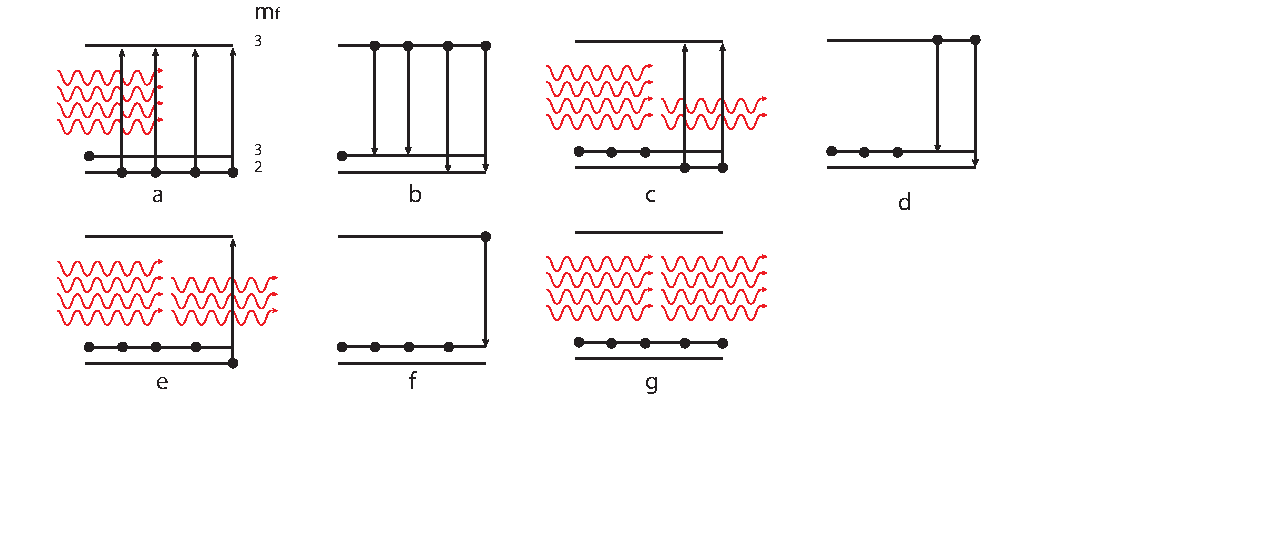
\includegraphics{figs/pumping}
  \caption{Optical pumping of Rb atoms with 795 nm light}
  \label{pumping}
\end{figure}

A visual description for de-pumping and zero-fielding can be seen in Figure \ref{rfing}. Now, all the Rb atoms have been trapped. What could cause a Rb atom to   absorb a photon again? There are two ways, the first is place the atoms in a zero-field situation so there is no more Zeeman splitting and they can absorb photons as usual. The second is de-pump the atoms into a lower state, now they can obey the selection rules and absorb photons.

How is a zero field situation created? Even if there is no magnetic field created in the lab Zeeman splitting will  occur because of the presence of the Earth's magnetic field. If one adjusts the magnetic field in a precise way the Earth's magnetic field can be canceled, thus creating a zero-field situation, shown in Figure \ref{rfing}b. 

How are atoms de-pumped? If the magnetic field is increased further then the Zeeman gap is also increased. What if the atoms are exposed to a second set of photons at the same time? The energy of these photons is
\begin{equation}
E = hf
\end{equation}
If the Zeeman energy gap is matched with the energy of the second set of photons then stimulated emission will occur, de-pumping a Rb atom so it is again able to absorb the higher energy exciting photons while obeying the selection rules, Figure \ref{rfing}d-\ref{rfing}e.
\begin{figure}[H]
  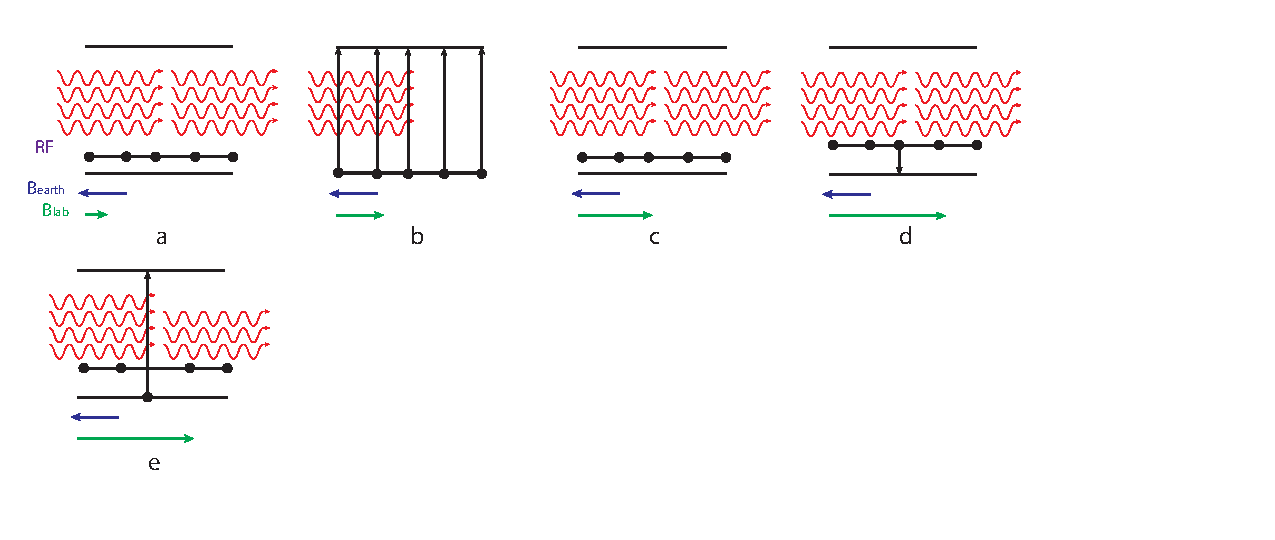
\includegraphics{figs/rfing}
  \caption{Zero-fielding and De-pumping Rb atoms with RF photons}
  \label{rfing}
\end{figure}

\section{Apparatus}
A schematic for our apparatus can be seen in Figure \ref{schematic}. We generate 795 nm light from a Rubidium lamp. The light is then manipulated and filtered so we get 795 nm circularly polarized light which is used to pump Rb atoms. After the light passes through the chamber we measured it's intensity with a detector.

Optical pumping and manipulation depend on a carefully controlled magnetic field. We generated the vertical and horizontal components of the lab's magnetic field with a pair of Helmholtz coils. Now we have trapped atoms, to de-pump them we require a second set of lower energy photons. We used Helmholtz coils to generate radio frequency photons shown in red, Figure \ref{schematic}g.

% magnetic field vs current
\begin{figure}[H]
  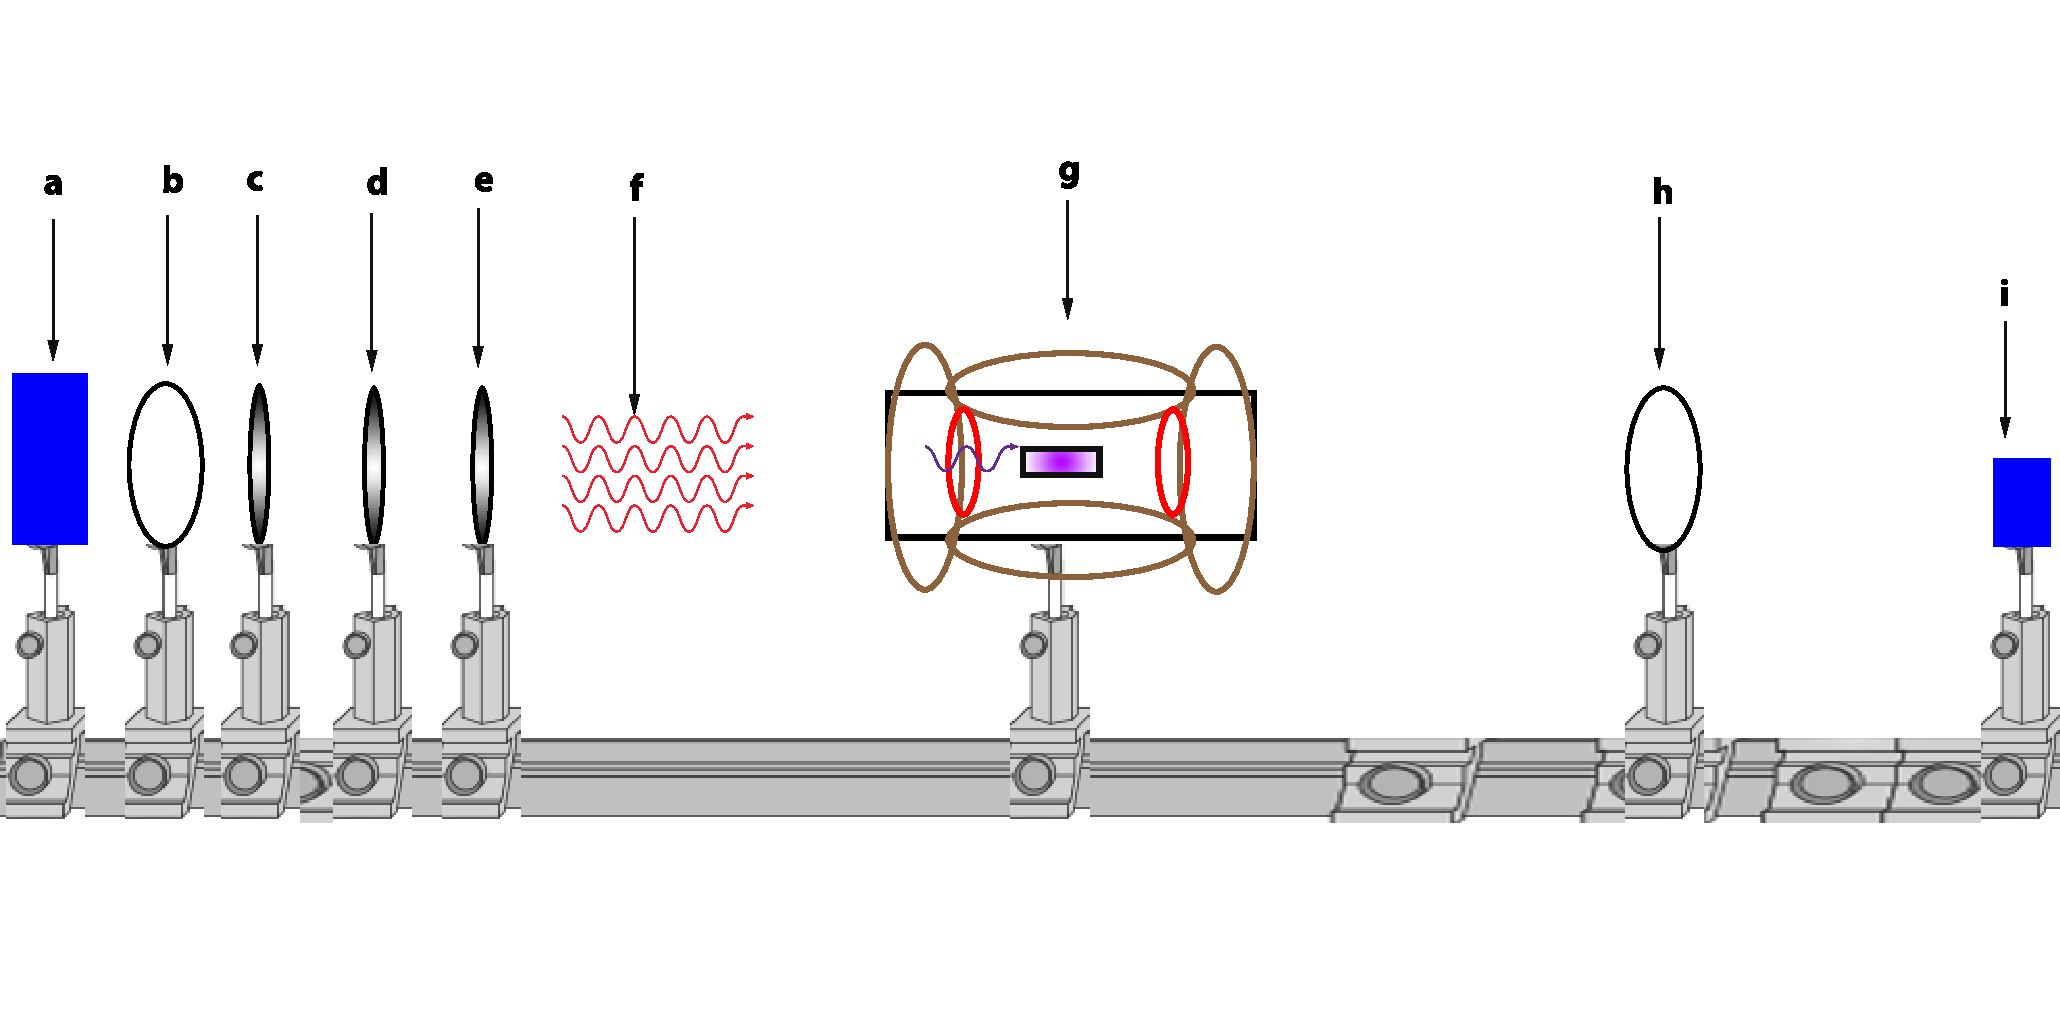
\includegraphics[totalheight=0.5\textwidth]{figs/apparatus}
  \caption{Experimental setup. \newline
a) Rubidium lamp \newline
b) lens, $f$ = 50 mm \newline
c) Interference filter \newline
d) Polarizer \newline
e) Quarter wave plate \newline
f) 795 nm right circularly polarized light \newline
g) Helmholtz coils, with rubidium chamber \newline
h) lens, $f$ = 50 mm \newline
i) Amplified photo-detector}
  \label{schematic}
\end{figure}


\section{Analysis}
What kind of behavior will a system of trapped atoms that is suddenly freed exhibit? It will absorb light, which is to say go from transparent to not transparent. We can measure and detect when this happens because the intensity of the light passing through the chamber will suddenly decrease. By sweeping through an increasing range of magnetic fields we can see when the magnetic field is just right to cause: a cancellation of Earth's magnetic field, stimulated emission of  $^{87}$Rb and stimulated emission of $^{85}$Rb, shown in Figure \ref{depumping}. What will happen if the radio frequency is increased? Now the Zeeman energy gap must be larger for stimulated emission to occur so we would see the two humps slide to the right.
% MATLAB by itself EPS
\begin{figure}[H]
  \includegraphics[totalheight=0.6\textwidth]{figs/depumping_final}
  \caption{Drop in light intensity caused by canceling Earth's magnetic field and de-pumping $^{85}$Rb and $^{87}$Rb}
  \label{depumping}
\end{figure}

Because we can measure the current through the Helmholtz coils and we know the required physical parameters of the coils we can measure the magnetic field. Because we know the energy of the RF photons we can measure the Zeeman energy gap. A plot and fit of the energy gap vs. magnetic field can be seen in Figures \ref{rb85line} and \ref{rb87line}. We determined the slope of the line and by applying Equation \ref{zeeman} we determined the Lande g-factors. Our results can be seen in Table \ref{result}. Taking the ratio we obtain $g^{\mathrm{exp}}_{87}$/$g^{\mathrm{exp}}_{85}$ = $1.5 \pm 0.1$ which agrees with the accepted value $g_{87}$/$g_{85}$ = 1.5, shown in Table \ref{result2}.
% MATLAB by itself EPS
\begin{figure}[H]
  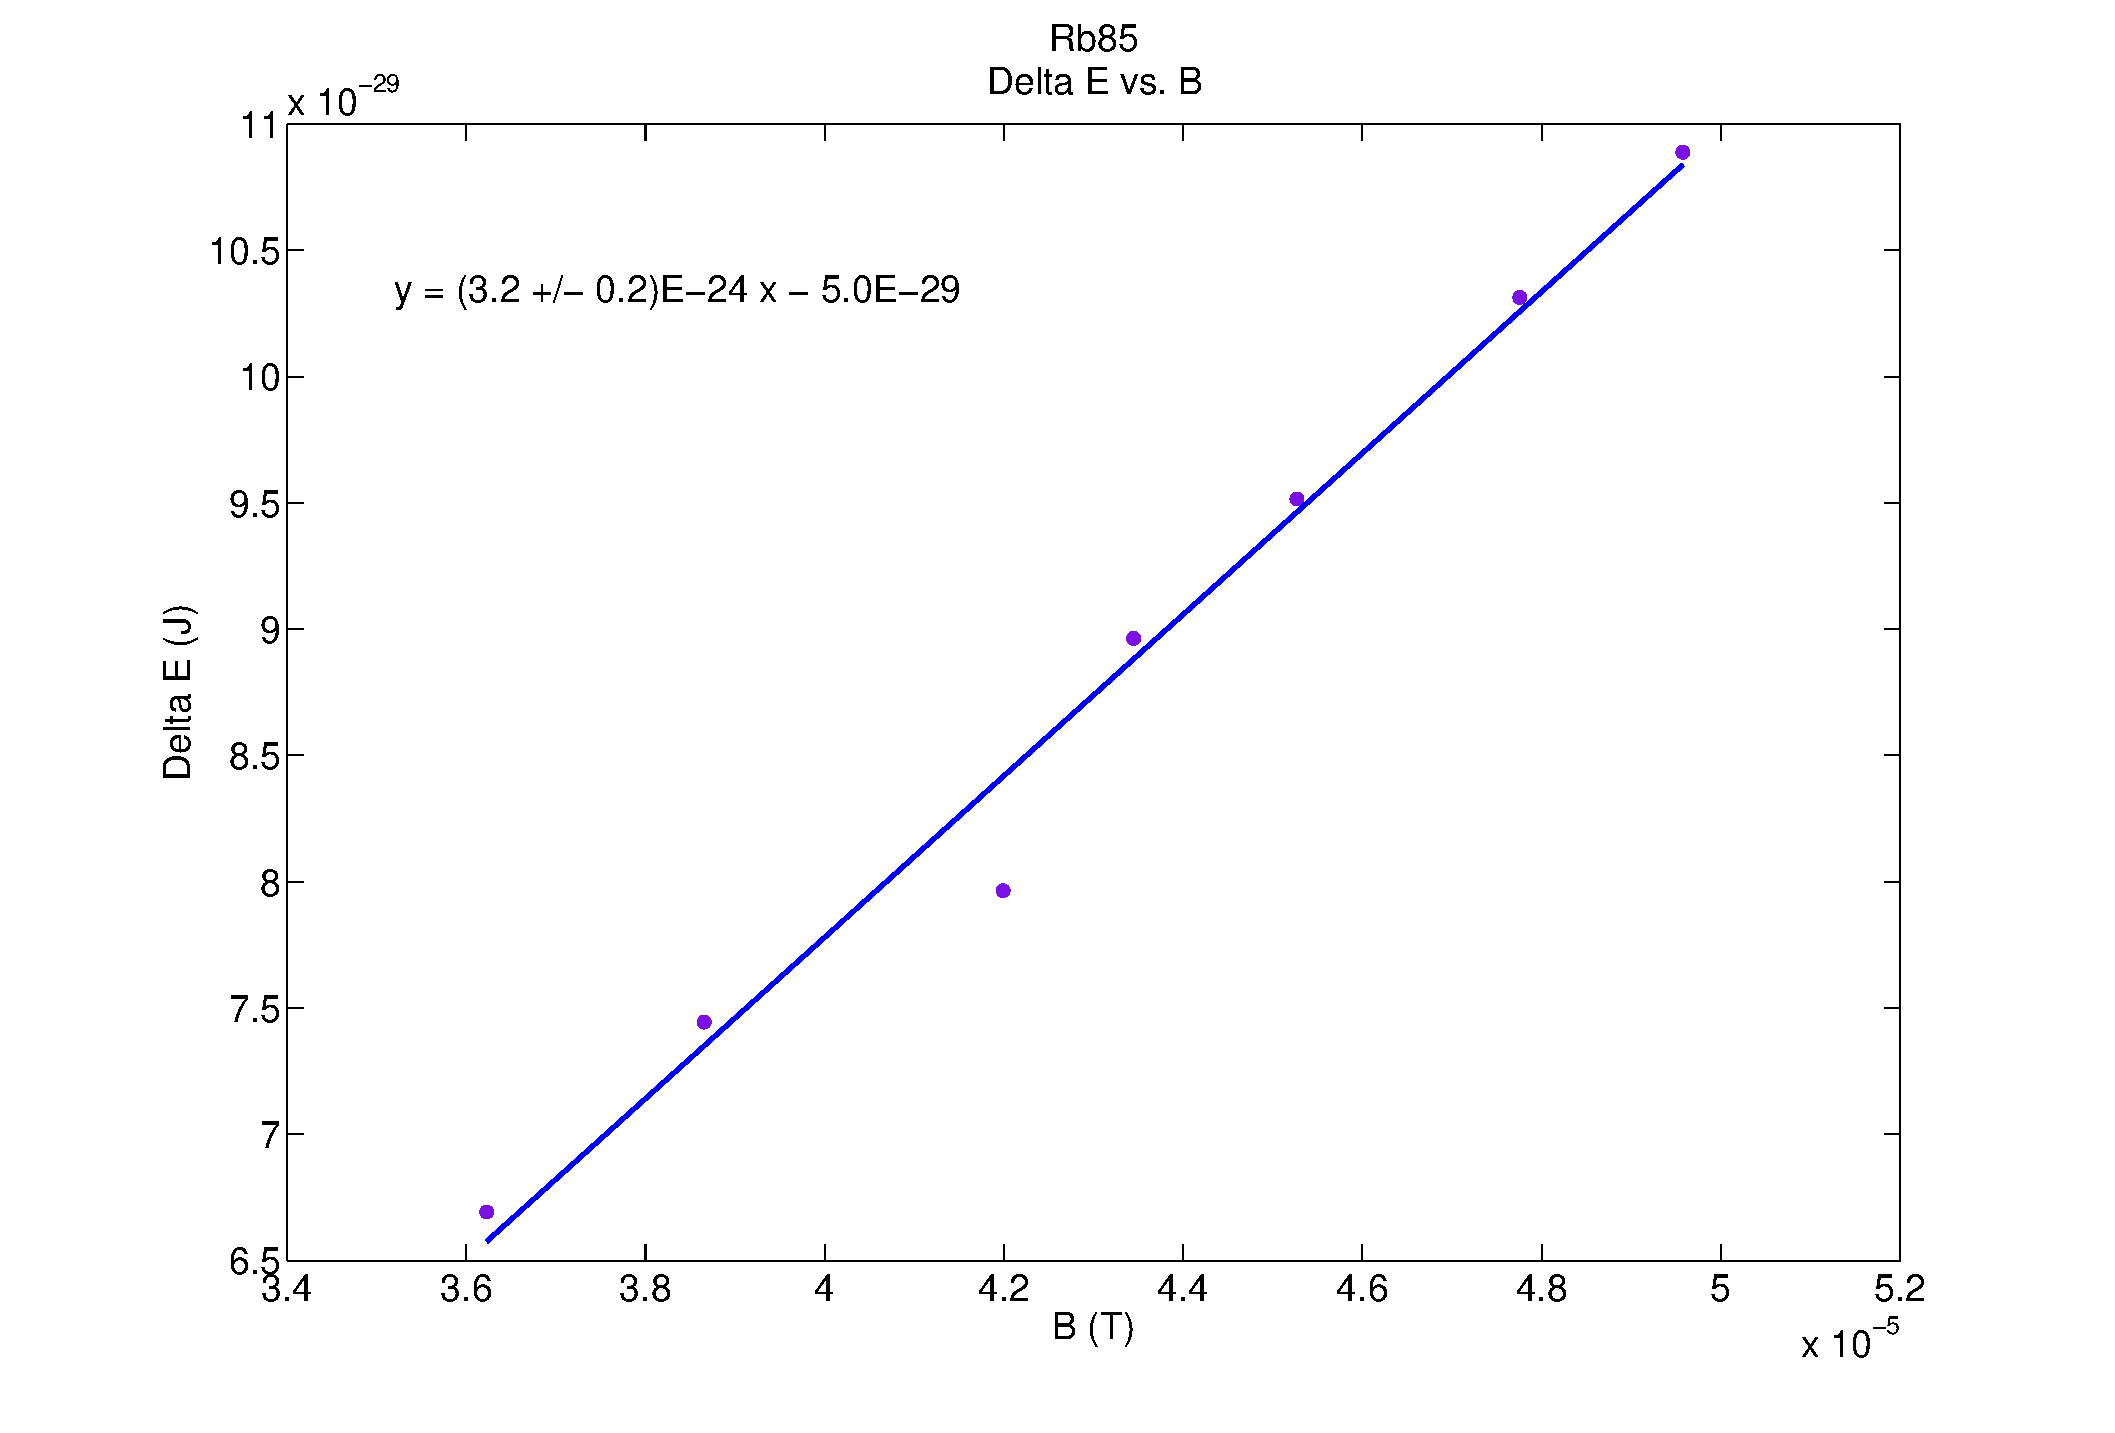
\includegraphics[totalheight=0.6\textwidth]{figs/rb85}
  \caption{Determining the slope of  $\Delta E$ vs. $B$  for  $^{85}$Rb}
  \label{rb85line}
\end{figure}

% MATLAB by itself EPS
\begin{figure}[H]
  \includegraphics[totalheight=0.6\textwidth]{figs/rb87}
  \caption{Determining the slope of $\Delta E$ vs. $B$  for  $^{87}$Rb}
  \label{rb87line}
\end{figure}

\begin{table}[H]
\caption{Experimental g-factors }
\begin{tabular}{c@{\hskip 1cm} c}
\hline\noalign{\smallskip}
Isotope & $g_{\mathrm{f}_{\mathrm{exp}}}$ \\
\hline\noalign{\smallskip}
$^{85}$Rb & $0.34 \pm 0.02$\\
$^{87}$Rb & $0.52 \pm 0.03$\\
\hline\noalign{\smallskip}
\end{tabular}
\label{result}
\end{table}

\begin{table}[H]
\caption{Experimental and Accepted g-factor ratio from \cite{mit} }
\begin{tabular}{c@{\hskip 1cm} c@{\hskip 1cm} c}
\hline\noalign{\smallskip}
Quantity & Experimental Value & Accepted Value \\
\hline\noalign{\smallskip}
$g_{87}$/$g_{85}$ & $1.5 \pm 0.1$ & 1.5 \\
\hline\noalign{\smallskip}
\end{tabular}
\label{result2}
\end{table}

\section{Conclusion}
We performed optical pumping to trap $^{85}$Rb and  $^{87}$Rb atoms. We measured the strength of an applied magnetic field and the intensity of light passing through the Rb vapor. We determined the Lande g-factors for each of the isotopes which agree with accepted values. We also observed our applied magnetic field cancel the Earth's magnetic field.



\begin{thebibliography}{99}

\bibitem{manual} Physics Dept., ``Optical Pumping'', Quantum Lab,
  California Polytechnic University, (2013).

\bibitem{wiki} ``Optical pumping'', Wikipedia: The Free Encyclopedia. Wikimedia Foundation, Inc., 05 December 2013. Web. wikipedia.org/wiki/Opticalpumping.


\bibitem{mit} A. Speranza, ``Optical Pumping of Rubidium Vapor'', MIT Physics Dept.,MIT University, (2013).


\end{thebibliography}

\end{document}
